\subsection{会員機能}
会員機能は，以下のような機能から構成されている．

\begin{itemize}
    \item ログイン・ログアウト
    \item 退会
    \item 問い合わせ
\end{itemize}


\subsubsection{ログイン・ログアウト}
事業者会員がGoogle認証を用いて、任意にログイン・ログアウトを行う機能．

ログイン機能では，事業者会員が Google アカウントを用いた認証によりシステムへログインする．

ログインの流れとしては，まず「利用規約に同意する」にチェックを入れ，「Google でログイン」を選択する．
その後，Google 認証画面へ遷移し，任意のアカウントを選択して認証を行う．
認証後，データベースへアクセスし，登録済みのアカウント情報と一致するかを照合する．
照合が成功した場合はログインを許可し，ホーム画面へ遷移する．


\begin{figure}[H]
    \centering
    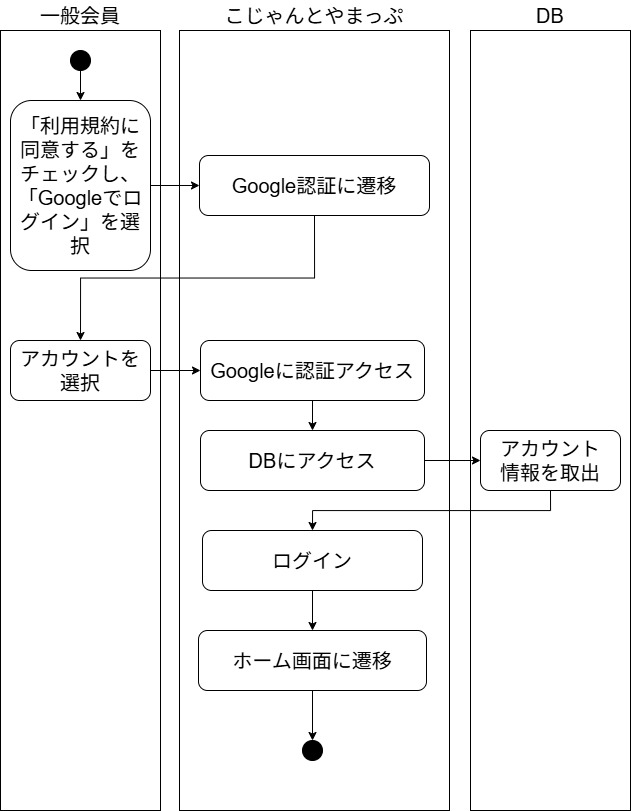
\includegraphics[scale=0.5]{sections/fig_account_business/account_bus1_1.jpg}
    \caption{ログイン}
    %\label{fig:pinpost_bus1_1}
\end{figure}

ログアウト機能では，すでにログインしている会員が任意のタイミングでログアウト操作を行うことができる．
ログアウト操作時にはまずログアウト画面を表示し，ユーザがキャンセルを選択した場合はホーム画面へ戻る．
ログアウトを確定した場合はセッション情報を無効化し，ログイン画面へ遷移する．


\begin{figure}[H]
    \centering
    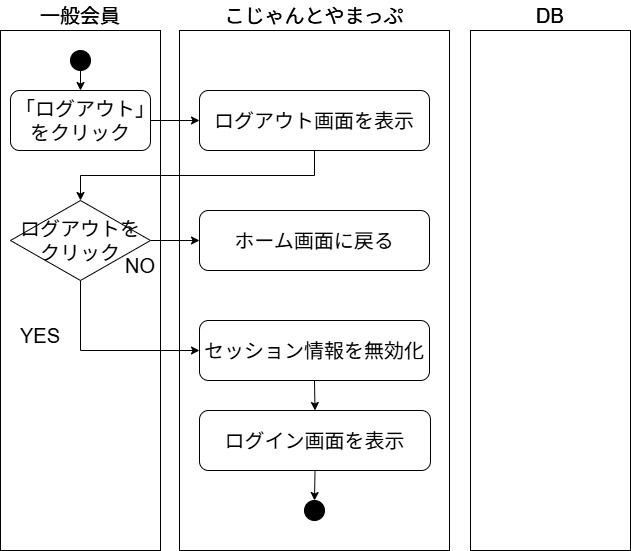
\includegraphics[scale=0.5]{sections/fig_account_business/account_bus1_2.jpg}
    \caption{ログアウト}
    %\label{fig:pinpost_bus1_1}
\end{figure}